\section{System Architecture}
As we previously said, our system is a simulator whose computation spreads
across multiple nodes.

\subsection{Macro components}

In order to easily reason about the system, we
divide it in three logical macro components.
An overall view of our architecture
is depicted in Figure \ref{fig:sd-sys-arch-overall}:

\begin{figure}[H]
  \centering
  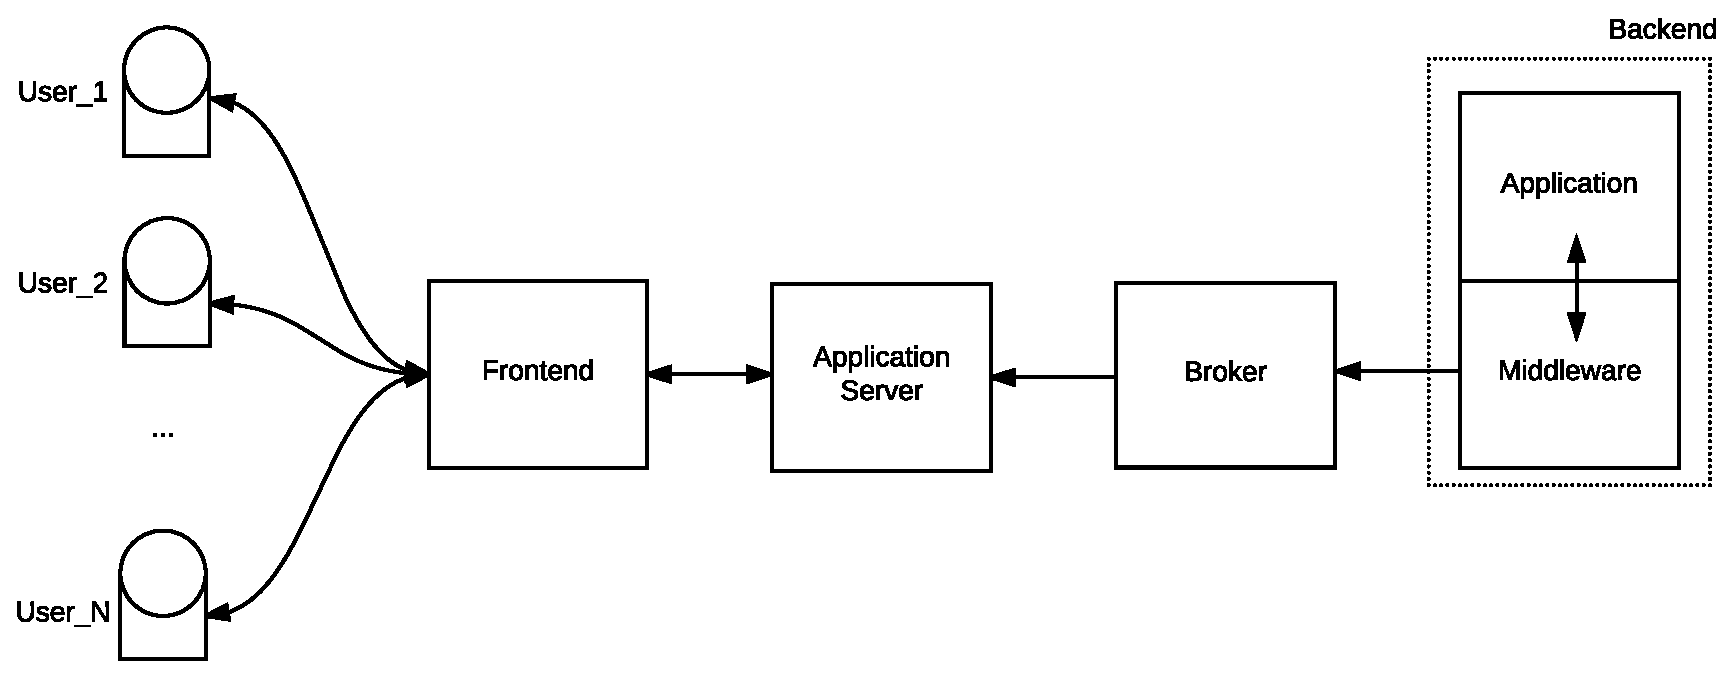
\includegraphics[scale=0.5,keepaspectratio]
    {images/solution/overall-arch.eps}
  \caption{Overall system architecture}
  \label{fig:sd-sys-arch-overall}
\end{figure}

As we can see from Figure \ref{fig:sd-sys-arch-overall}, the system consists of:

\begin{itemize}
  \item \textbf{Backend:} comprises the \textbf{Application} and the
    \textbf{Middleware} layer;
  \item \textbf{Message Broker:} which is responsible to filter, format
    and eventually enrich the messages which flow between the other components.
%    Please keep in mind that this component is \textit{not} RabbitMQ itself,
%    but an architectural component we decided to put in our system;
  \item \textbf{Frontend:} split in:
  \begin{itemize}
    \item \textbf{Application Server:} which is responsible of handling
      information generated by the backend and to serve it to the viewer;
    \item \textbf{Viewer:} which offers the streaming services to end users.
  \end{itemize}
\end{itemize}

The backend and
the application server are loosely coupled. They communicate using a
publish-subscribe mechanism. Thus, their
communication is managed through a set of different queues.
The application server keeps very little information for
each connected user. It is linked to a persistent separated component
which will eventually store set of specific messages
(if a persistent consumer is enabled).


Each layer should be transparent to the other layers. Thus,
the middleware has to be unaware
of the specific domain of our application logic.
Thus, the application should expose an interface for the generic operations of
a computational node, like boot and shutdown.


The message broker can scale transparently to the other components: if we
were to replicate application servers to cope with a rising amount of
sessions, we could instantiate more than one broker per city (actually, one
per application server connected to a specific city).
Also, these brokers provide a useful means to enrich the topic of the messages
by inspecting their content. Therefore, lighter versions of the
same incoming messages, but with a more specific topic, will be sent out by the
broker towards to the application server.

Each one of these architectural macro components can be distributed as well: we
focused our efforts on distributing the backend over multiple computation nodes
by using a \textit{2D-wrap-around topology}.
We thought this is an interesting approach to distribute our system since it
fits perfectly the way we can divide a simulated city, besides the fact this is
a topology which scales well when it comes to distribute network traffic.

In particular, we think this topology fits our needs. Indeed, the
most frequent application-level actions are
represented by a traveler which moves from a district to an
adjacent one to continue its travel. Obviously this actions span over
multiple nodes.

Therefore, if adjacent backend nodes contain adjacent districts, we are able to
avoid a significant amount of unnecessary network traffic. In Figure
\ref{fig:sd-sys-arch-topology} we show a sample city in which each district
$D_i$ is a backend node, the edges starting from each district are the links
between backend nodes:

\begin{figure}[H]
  \centering
  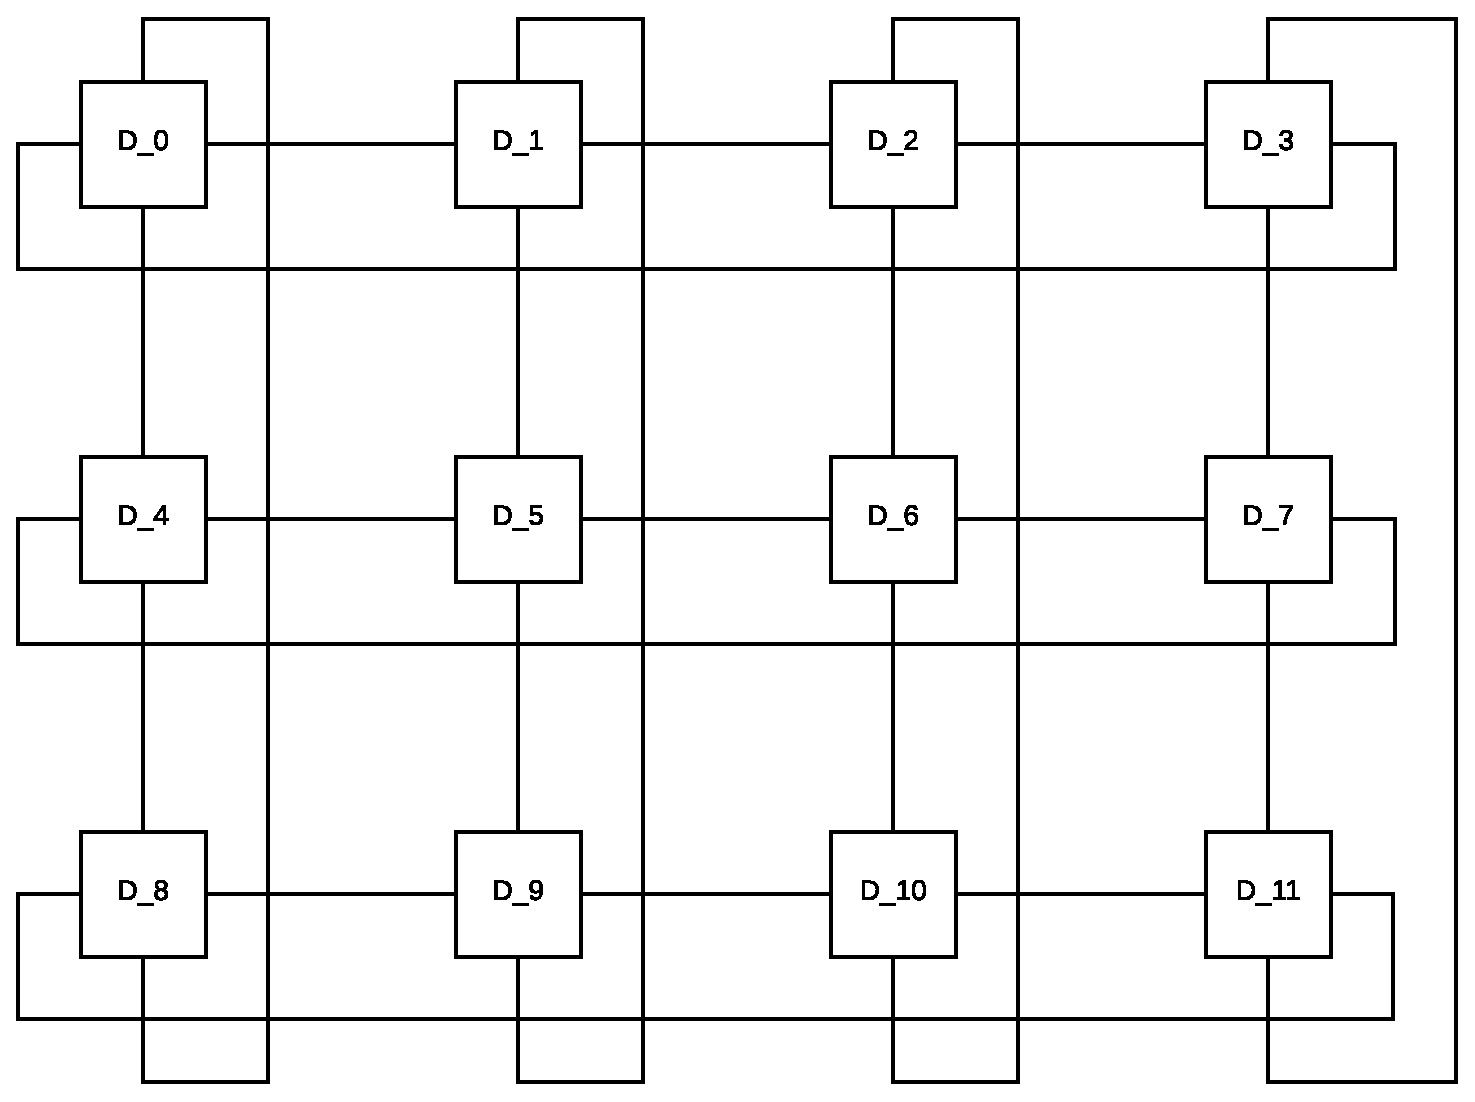
\includegraphics[scale=0.5,keepaspectratio]
    {images/solution/topology.eps}
  \caption{Sample topology for our system}
  \label{fig:sd-sys-arch-topology}
\end{figure}


\subsection{Microservice architecture}

We further decoupled each macro component into a set of isolated services
which communicate by exchanging messages. The decoupling into micro isolated
services enables our system to scale horizontally. Indeed, each service is wrapped
into a container. Thus, we can replicate
the services as needed by specifying the maximum number of replicas
for each of them.
It is the major advantage
of a microservice architecture.
The drawback consists in the complexity to manage a set of decoupled
services instead of a monolithic one.


Due to this complexity
we need an external entity which
will have the responsibility to manage and monitor all the services:
e.g., when a node crashes it should schedule another node or reactivate it
transparently to the end user.
The orchestrator will
manipulate the \textit{service} level, without knowing anything about
what is inside each node. This is extremely important because it
lets us to assign
a single responsibility to the orchestrator and clearly
separate the services from it.


The Figure \ref{fig:sd-sys-arch-micro} represents how we have decoupled
the components as microservices. However, we have not been able to decompose the
frontend macro component as we initially designed to do.

\begin{figure}[H]
  \centering
  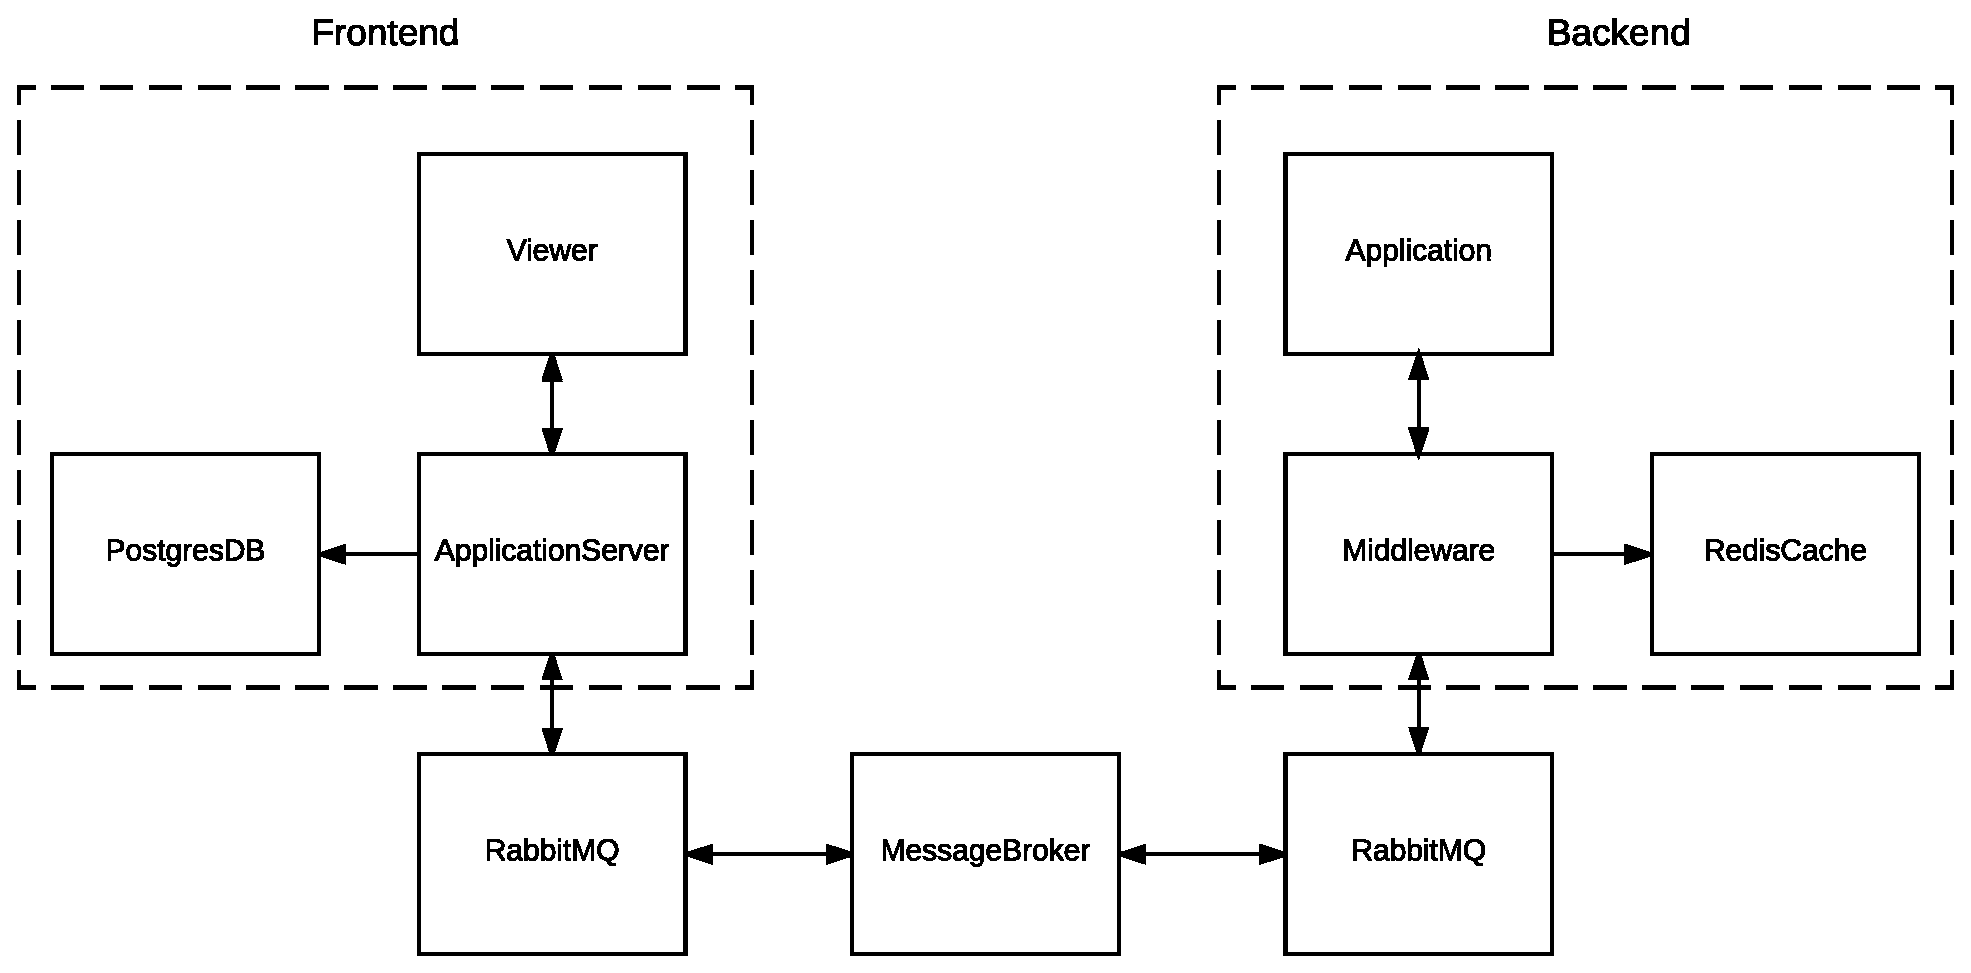
\includegraphics[scale=0.5,keepaspectratio]
    {images/solution/microservices.eps}
  \caption{The microservice architecture of the city system}
  \label{fig:sd-sys-arch-micro}
\end{figure}


\subsection{Deployment}
In light of the above, we designed the deployment of our system. Even
if a single city simulation would be composed of all the services depicted
in Figure
\ref{fig:sd-sys-arch-micro}, it is not reasonable to instantiate all of them
each time a new simulation for a city is requested.
We instead propose a different approach: multiple users share the same frontend
(regardless of the fact they are consuming the same simulation) and all the
services from the message broker to the application will vary for each city.
Indeed, each city is represented by a different configuration file which
describes
all of its districts. Furthermore, each district is mapped to a different
service.
Finally, we identify the RabbitMQ broker as the Application Server endpoint for
the MessageBrokers of the different city instances.

Our proposed solution has a visual representation in Figure
\ref{fig:ovrl-deployment}, in which we used the following notation:

\begin{itemize}
  \item \textbf{City\_X:} instance of a city, which is composed of a Backend,
    a MessageBroker and the RabbitMQ broker between them;
  \item \textbf{RabbitMQ Broker:} node which basically provides bidirectional
    communication between the cities and the frontend. Cities send events to
    the frontend, whereas the latter starts city instances by means of this
    broker;
  \item \textbf{Frontend:} Node which is composed of the ApplicationServer and
    the Viewer. It keeps track of which city simulations are currently
    running and serves live streaming services to end users.
\end{itemize}

\begin{figure}[H]
  \centering
  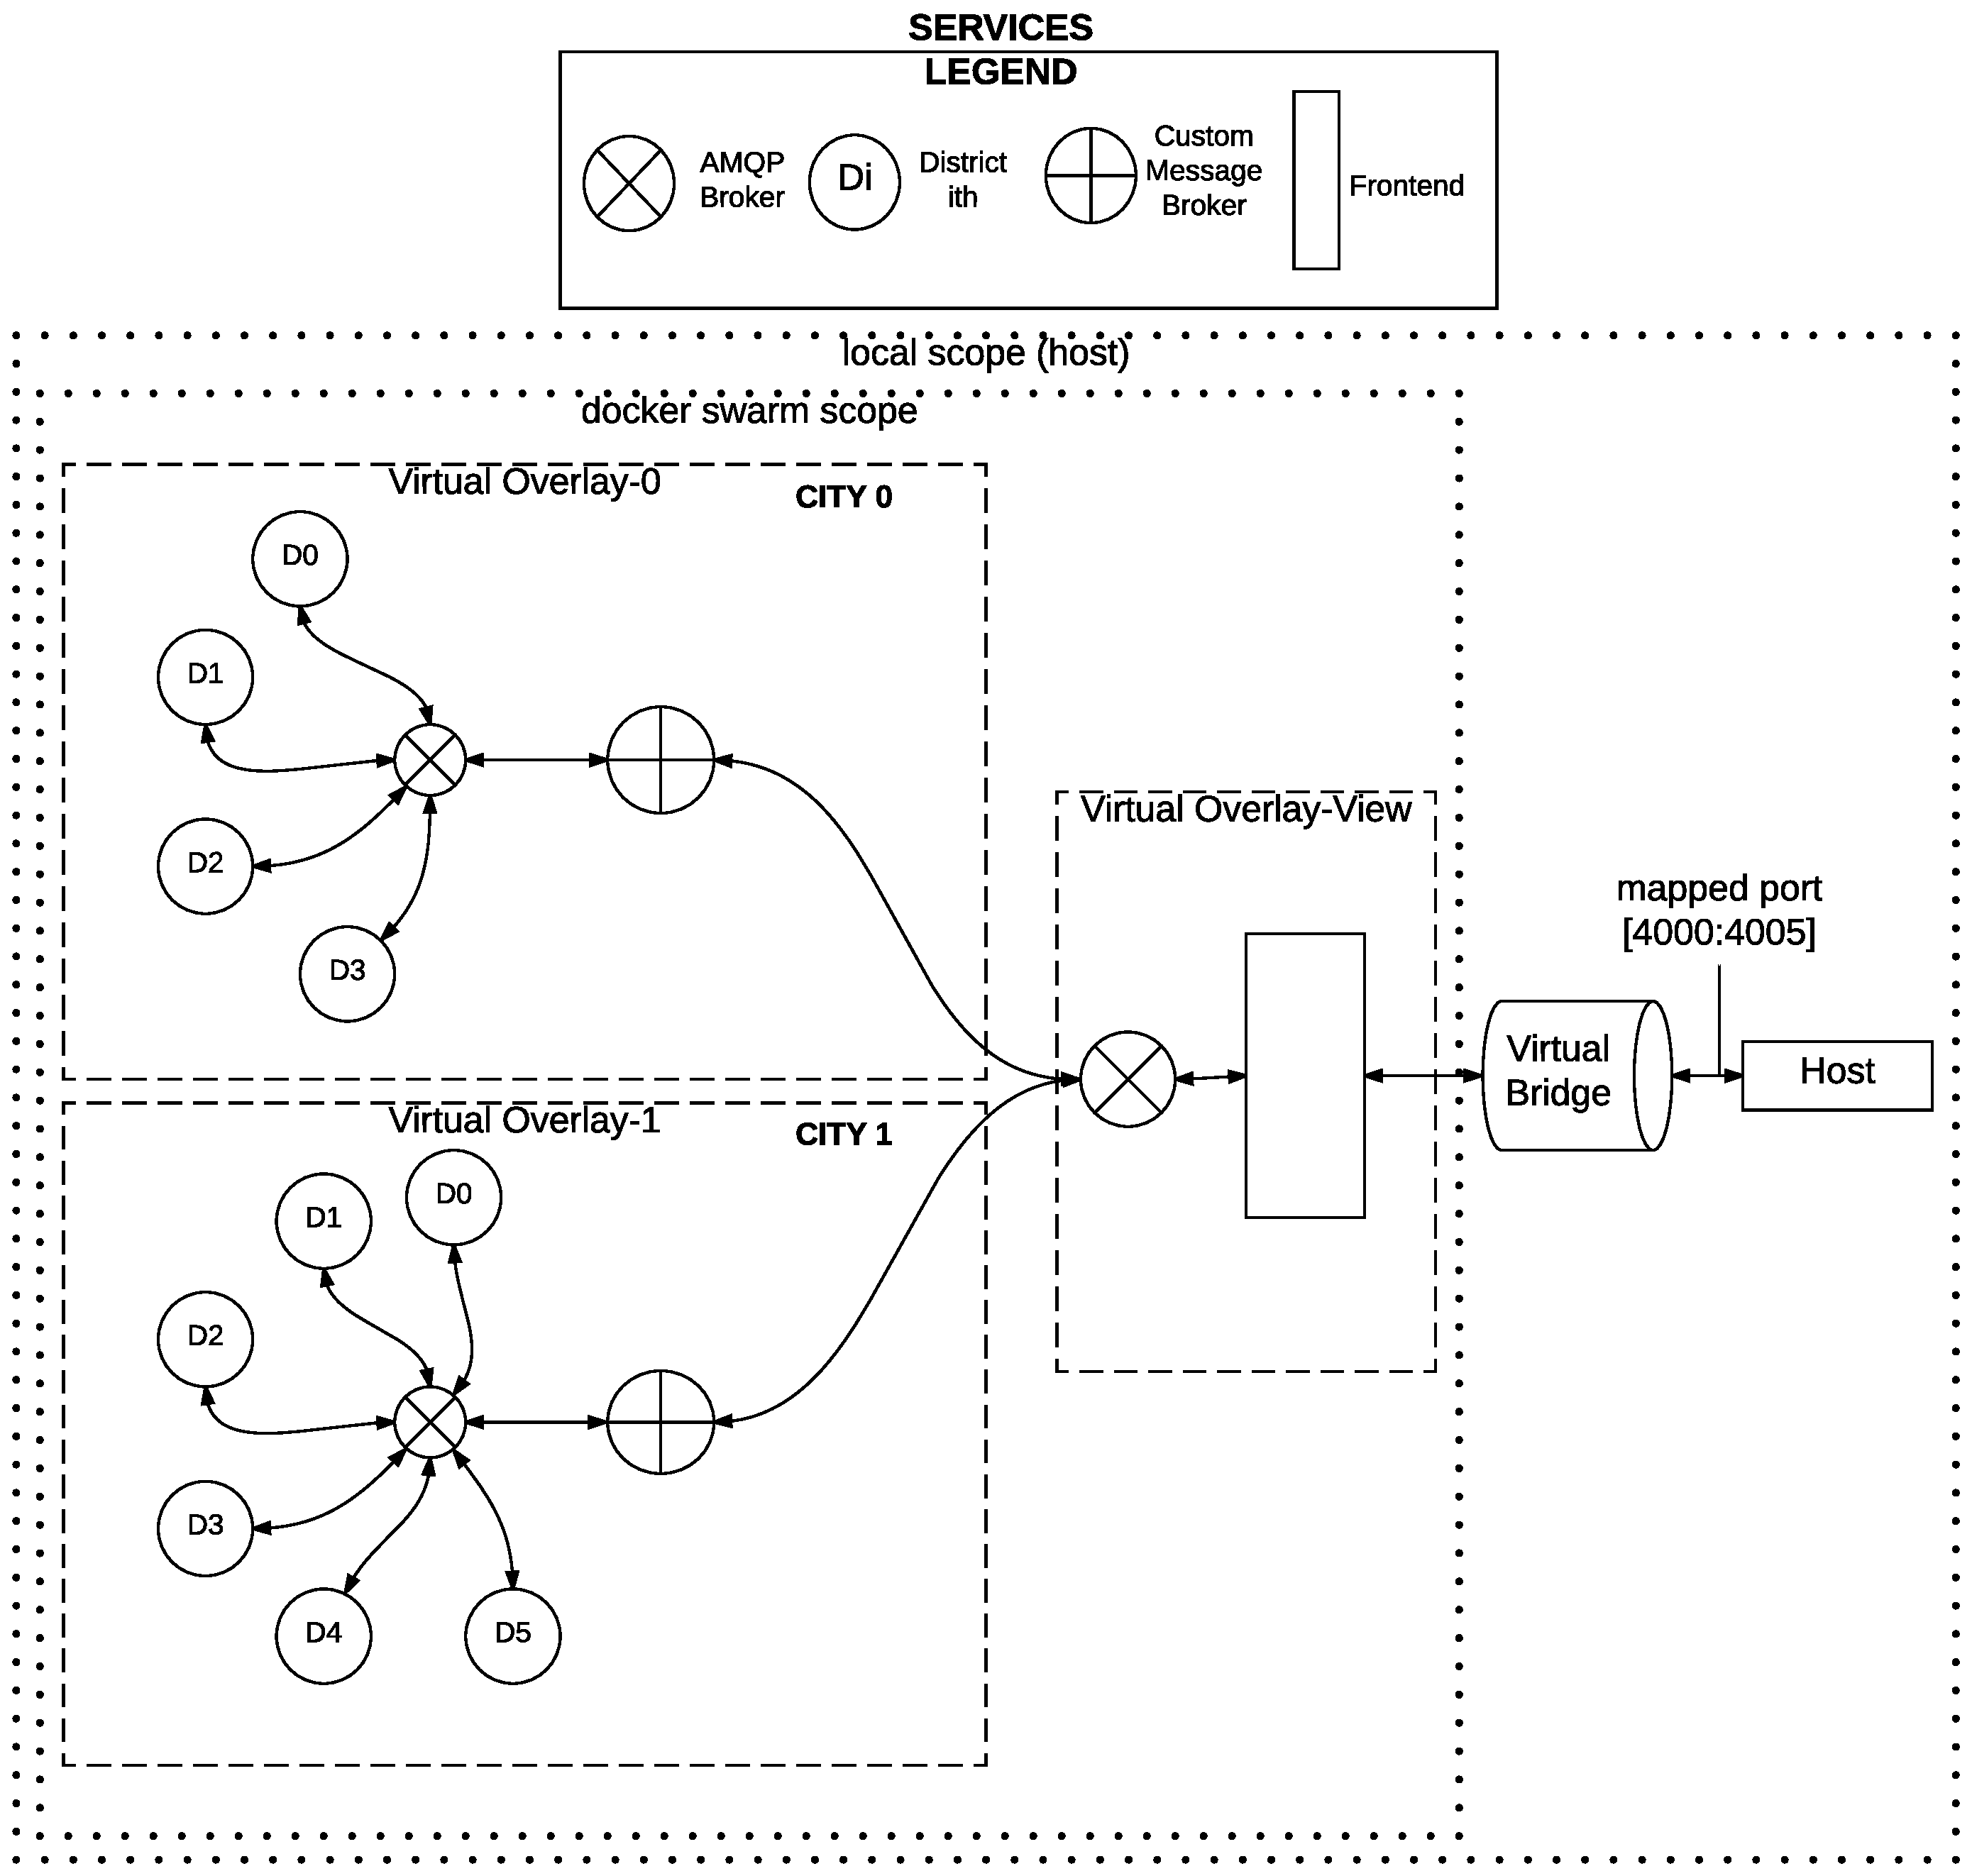
\includegraphics[scale=0.25,keepaspectratio]
    {images/overall/deploy.eps}
  \caption{System deployment}
  \label{fig:ovrl-deployment}
\end{figure}
